\documentclass[reprint, aps, 12pt, floatfix]{revtex4-2}

\usepackage{graphicx, amsmath, gensymb, amssymb, units, dcolumn, bm, pgfplots, setspace, placeins, caption}
\pgfplotsset{compat=1.18}

\begin{document}

\title{Investigating Two-Step Perfect Quantum State Transfer in Continuous-Time Quantum Walks on Small Graphs}
\author{Nathan Ngo \& Supervisor:\;David Feder}
\date{\today}

\begin{abstract}
\singlespacing
This thesis investigates two-step perfect quantum state transfer (PST) in continuous-time quantum walks, in which a quantum state is transferred through two sequential unitary evolutions. Using numerical optimization via TensorFlow’s Adam algorithm, an unbounded family of two-step PST solutions was identified on the weighted path graph P$_4$ between nodes 1 and 4; this family was subsequently found to also support one-step PST. On the weighted cycle graph C$_3$, two-step state transfer from node 1 to node 2 achieved infidelity below $10^{-12}$, strongly indicating the presence of PST; equivalent fidelity was later observed under a one-step protocol as well. In contrast, for state transfer from node 1 to node 3 on weighted C$_3$, one-step evolution consistently failed to reach high fidelity, while the two-step approach yielded infidelity below $10^{-12}$—demonstrating a clear advantage. These results highlight the role of the two-step protocol in enabling near-perfect or perfect state transfer in cases where one-step dynamics are insufficient, thereby expanding the class of graph structures suitable for quantum communication tasks.
\end{abstract}


\maketitle
\singlespacing

\section{Introduction}
Perfect quantum state transfer (PST) refers to the process of transferring quantum information between locations with perfect fidelity, a critical requirement in quantum computing and communication systems~\cite{BoseSougato2003Qcta}. The approach of two-step PST, while less understood than one-step PST, offers increased flexibility and potential advantages for quantum networks.

\section{Background and Motivation}

In classical random walks, a walker moves probabilistically from one point to another. In continuous-time classical random walks, the walker evolves according to partial differential equations like the diffusion equation:
\begin{equation}
    \frac{\partial P(x,t)}{\partial t} = D \frac{\partial^2 P(x,t)}{\partial x^2},
\end{equation}
where $P(x,t)$ is the probability distribution at position $x$ and time $t$, and $D$ is the diffusion constant.

By contrast, continuous-time quantum walks (CTQWs) are governed by the time-dependent Schrödinger equation:
\begin{equation}
    i\hbar\frac{\partial\psi(x,t)}{\partial t}=-\frac{\hbar^2}{2m}\frac{\partial^2\psi(x,t)}{\partial x^2},
\end{equation}
and the evolution of a quantum state on a graph is given by
\begin{equation}
    |\psi(t)\rangle = e^{-\nicefrac{iHt}{\hbar}} |\psi(0)\rangle,
\end{equation}
where $ |\psi(t)\rangle $ is the quantum state of the walker and $H$ is the adjacency matrix of the graph~\cite{FarhiEdward1998Qcad}.

A rare phenomenon in CTQW—perfect quantum state transfer—is vital for quantum networks, where information can be transferred with perfect fidelity~\cite{BoseSougato2003Qcta}, meaning no loss of information. Theory on one-step PST, where the state is transferred directly between two nodes in a single step, is already well-established. However, since PST is only possible on a limited set of graphs~\cite{Kendon:2011:1546-1955:422}, alternative approaches must be explored. Two-step PST, which involves an intermediate state between two sequential quantum walk evolutions, could potentially enable more complex graph structures. This increased flexibility may enhance the robustness of quantum communication systems. As quantum technologies scale, understanding and leveraging two-step PST could lead to more efficient network designs and higher reliability. A sample calculation showing the analytical solution of one-step PST on P$_2$ is provided in Appendix A.

\section{Literature Review}
Continuous-time quantum walks have been extensively studied, with research highlighting their potential for applications in quantum computing~\cite{KempeJ2003QrwA}. Tsuji et al.~\cite{TsujiYuta2018QIGW} discussed how quantum interference in CTQWs enables efficient state transfer processes. Coutinho et al.~\cite{CoutinhoGabriel2022Qwdn} explored the limitations of quantum walks in bridging nodes in graph structures, specifically analyzing the restrictions imposed by ``bridge'' in graphs. Godsil et al.~\cite{GodsilChris2012Nnoc} provided a comprehensive review of state transfer on graphs, showing that certain symmetric graph structures allow for PST. While one-step PST has been widely examined, research on two-step PST remains absent. The underlying conditions for two-step PST to occur are still poorly understood. Since two-step PST was not previously recognized as a distinct mechanism, it had not been actively considered in the design or analysis of quantum networks. As a result, its potential advantages and constraints remain largely unexplored in the existing literature.

\subsection{Unweighted Small Graphs}
PST is highly sensitive to the structural properties of the underlying graph. In particular, certain unweighted small graphs—such as path and cycle graphs—exhibit intrinsic limitations that prevent one-step PST.

For unweighted path graphs P$_n$, one-step PST is possible only in a few specific instances. Notably, PST can occur only when $ n \leq 3 $; beyond three vertices, the condition required for PST breaks down, and the phenomenon no longer occurs~\cite{Kendon:2011:1546-1955:422}.

Unweighted cycle graphs C$_n$ are similarly constrained. Among these, only the four-vertex cycle graph C$_4$ supports one-step PST. All other unweighted cycles—including C$_3$ and cycles with more than four vertices—fail to exhibit one-step PST~\cite{Kendon:2011:1546-1955:422}.

\subsection{Pretty Good State Transfer (PGST)}
In contrast to PST where the quantum state is transferred from one vertex to another with fidelity exactly equal to 1 at a specific time, pretty good state transfer (PGST) has a more relaxed requirement. PGST is a state transfer with fidelity arbitrarily close to 1, without it being exactly 1. It is much more abundant and flexible across a wide range of graph structures.

PGST has been observed in families of graphs where PST is either impossible or highly constrained. For example, while unweighted path graphs P$_n$ only admit PST for $n\leq3$, many longer unweighted paths admit PGST between their endpoints~\cite{GodsilChris2012Nnoc}. Similarly, Cartesian products of path graphs can exhibit PGST among their corner vertices, even though they may not allow PST~\cite{chan2023prettygoodstatetransfer}.

One of the key trade-offs in PGST is the relationship between fidelity and transfer time. As shown by Banchi et al., achieving a fidelity closer to 1 typically requires an exponentially longer evolution time~\cite{10.1063/1.4978327}. This distinguishes PGST from PST not only in precision but also in practicality—while PGST offers greater structural flexibility, it may be less suitable for time-sensitive quantum communication tasks.

PST is ideal for perfect, deterministic quantum information transfer but only occurs in highly symmetric or specifically constructed graphs. PGST, on the other hand, is more ubiquitous and structurally tolerant but requires accepting approximate fidelity and potentially long waiting times.

\section{Methodology}
The methodology employed can be summarized in five key steps: graph selection, optimizer implementation, identification of mathematical structures, analytical verification, and pattern recognition.

\subsection{Graph Selection}
Two graphs were selected for this study: the path graph P$_4$ (Fig.~\ref{fig:general p4}) and the cycle graph C$_3$, each with real-valued edge weights. The path graph P$_4$, consisting of four vertices connected linearly, was chosen due to the existence of two known configurations that exhibit PST from node 1 to node 4 (Fig.~\ref{fig:p4 case 1} and Fig.~\ref{fig:p4 case 2}). It has been shown that PST can occur on a weighted P$_4$ when the edge weights are carefully engineered to specific values. These known cases motivated a broader search for families of graphs exhibiting similar PST behavior.

\begin{figure}
    \centering
    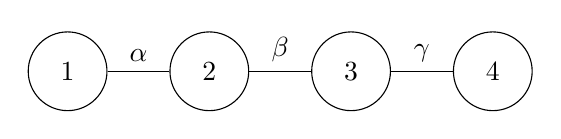
\begin{tikzpicture}[scale=0.9]
        % Draw nodes
        \node[circle, draw, fill=white, minimum size=1cm] (1) at (0,0) {1};
        \node[circle, draw, fill=white, minimum size=1cm] (2) at (2,0) {2};
        \node[circle, draw, fill=white, minimum size=1cm] (3) at (4,0) {3};
        \node[circle, draw, fill=white, minimum size=1cm] (4) at (6,0) {4};
        
        % Draw connections
        \draw[-] (1) -- (2) node[midway, above] {$\alpha$};
        \draw[-] (2) -- (3) node[midway, above] {$\beta$};
        \draw[-] (3) -- (4) node[midway, above] {$\gamma$};
            
        % Labels
        \node[below] at (1) {};
        \node[below] at (2) {};
        \node[below] at (3) {};
        \node[below] at (4) {};
    \end{tikzpicture}
    \caption{\small The path graph P$_4$ with four vertices and three edges labeled by real-valued weights $ \alpha, \beta, \gamma \in \mathbb{R} $.}
    \label{fig:general p4}
\end{figure}

\begin{figure}
    \centering
    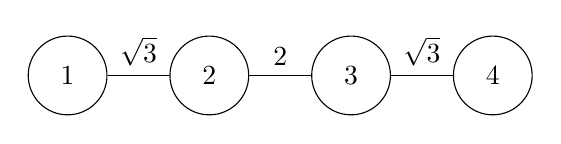
\begin{tikzpicture}[scale=0.9]
        % Draw nodes
        \node[circle, draw, fill=white, minimum size=1cm] (1) at (0,0) {1};
        \node[circle, draw, fill=white, minimum size=1cm] (2) at (2,0) {2};
        \node[circle, draw, fill=white, minimum size=1cm] (3) at (4,0) {3};
        \node[circle, draw, fill=white, minimum size=1cm] (4) at (6,0) {4};
        
        % Draw connections
        \draw[-] (1) -- (2) node[midway, above] {$\sqrt{3}$};
        \draw[-] (2) -- (3) node[midway, above] {$2$};
        \draw[-] (3) -- (4) node[midway, above] {$\sqrt{3}$};
            
        % Labels
        \node[below] at (1) {};
        \node[below] at (2) {};
        \node[below] at (3) {};
        \node[below] at (4) {};
    \end{tikzpicture}
    \caption{\small One of the two known PST configurations on the path graph P$_4$, with edge weights $\sqrt{3}$, $2$, and $\sqrt{3}$.}
    \label{fig:p4 case 1}
\end{figure}

\begin{figure}
    \centering
    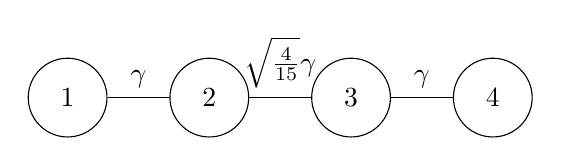
\begin{tikzpicture}[scale=0.9]
        % Draw nodes
        \node[circle, draw, fill=white, minimum size=1cm] (1) at (0,0) {1};
        \node[circle, draw, fill=white, minimum size=1cm] (2) at (2,0) {2};
        \node[circle, draw, fill=white, minimum size=1cm] (3) at (4,0) {3};
        \node[circle, draw, fill=white, minimum size=1cm] (4) at (6,0) {4};
        
        % Draw connections
        \draw[-] (1) -- (2) node[midway, above] {$\gamma$};
        \draw[-] (2) -- (3) node[midway, above] {$\sqrt{\frac{4}{15}}\gamma$};
        \draw[-] (3) -- (4) node[midway, above] {$\gamma$};
            
        % Labels
        \node[below] at (1) {};
        \node[below] at (2) {};
        \node[below] at (3) {};
        \node[below] at (4) {};
    \end{tikzpicture}
    \caption{\small The second of the two known PST configurations on the path graph P$_4$, with edge weights $\gamma$, $\sqrt{\nicefrac{4}{15}}\,\gamma$, and $\gamma$ where $\gamma\in\mathbb{R}$.}
    \label{fig:p4 case 2}
\end{figure}

The cycle graph C$_3$, a triangle with three vertices and three edges (Fig.~\ref{fig:general c3}), was also studied. Unlike P$_4$, there are no known instances of PST in any weighted C$_3$ when constrained to real edge weights; known cases typically involve imaginary weights. This absence provided motivation to investigate whether real-weight solutions could be discovered.

\begin{figure}[t]
    \centering
    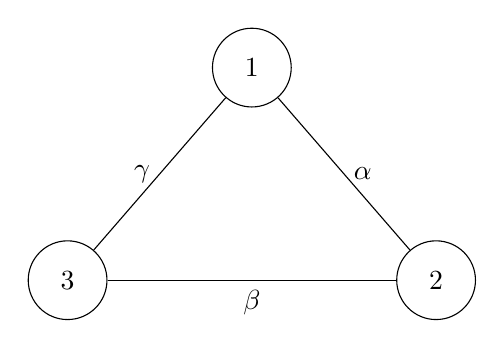
\begin{tikzpicture}[scale=0.9]
        % Draw nodes
        \node[circle, draw, fill=white, minimum size=1cm] (1) at (0,1.5) {1};
        \node[circle, draw, fill=white, minimum size=1cm] (2) at (2.6,-1.5) {2};
        \node[circle, draw, fill=white, minimum size=1cm] (3) at (-2.6,-1.5) {3};
        
        % Draw connections
        \draw[-] (1) -- (2) node[midway, right] {$\alpha$};
        \draw[-] (2) -- (3) node[midway, below] {$\beta$};
        \draw[-] (3) -- (1) node[midway, left] {$\gamma$};
            
        % Labels
        \node[below] at (1) {};
        \node[below] at (2) {};
        \node[below] at (3) {};
    \end{tikzpicture}
    \caption{\small The cycle graph C$_3$ with three vertices and three edges labeled by real-valued weights $ \alpha, \beta, \gamma \in \mathbb{R} $.}
    \label{fig:general c3}
\end{figure}

\subsection{Optimizer Implementation}
A numerical optimization approach was used to search for two-step PST solutions. The optimizer was implemented in Python using the TensorFlow framework, with the Adam optimizer~\cite{kingma2017adammethodstochasticoptimization} selected to maximize the fidelity of state transfer.

The optimization variables were the edge weights before and after adjustments, as well as the runtimes before and after adjustments. The objective was to find real-valued edge weights and runtimes such that the fidelity of state transfer approached unity. The output of the optimization process consisted of lists of irrational numbers representing the optimized edge weights and runtimes.

\paragraph{Challenges}
A significant challenge encountered in the optimization procedure arises from the presence of pretty good state transfer in the system. The existence of PGST leads to a highly complex optimization landscape characterized by an abundance of local minima. These local minima pose a serious obstacle to the optimizer. In many cases, the optimizer converges to one of these PGST-induced minima, where the fidelity is very close to one but never reaches exactly one. Since the objective of this project is to identify PST solutions, any fidelity value less than one is insufficient, regardless of how small the difference may be. The optimizer frequently becomes trapped in these local minima, and the gradient information alone is not enough to guide the search towards a global minimum corresponding to perfect fidelity.

To address this issue, alternative optimization algorithms that incorporate the concept of momentum were also considered. Momentum-based methods, such as stochastic gradient descent with momentum or Nesterov accelerated gradient, are designed to help the optimizer escape shallow local minima by adding an inertial term that allows the algorithm to continue moving in the same direction even when gradients vanish. However, in this project, these momentum-based methods proved ineffective. The local minima are not merely shallow basins; rather, they are steep and well-defined, with fidelity values that are arbitrarily close to, but strictly less than, one. As a result, no amount of momentum is sufficient to overcome the sharp gradient walls surrounding these local minima.

Another major limitation of the optimization procedure is its computational efficiency. Due to the large number of variables, the complexity of the optimization landscape, and the precision required to identify PST solutions, the convergence rate is exceedingly slow. Obtaining a single valid solution typically requires several hours of computation. Furthermore, generating a complete list of approximately ten distinct solutions can take over a full day of continuous computation. This computational burden places practical constraints on the scalability of the method and limits the number of solutions that can be feasibly obtained.

\paragraph{Solutions}
To address the difficulties posed by the large number of local minima induced by PGST, a stagnation detection mechanism was incorporated into the optimization procedure. This mechanism continuously monitors the improvement in the fidelity value over successive iterations. Specifically, if the rate of improvement in fidelity falls below a predefined threshold for a certain number of iterations, the optimizer interprets this behavior as an indication of stagnation. When stagnation is detected, the system introduces a Gaussian random perturbation to all optimization variables, effectively resetting the search process to a different region of the parameter space. This strategy is designed to escape from local minima associated with PGST and increase the likelihood of converging to a global minimum corresponding to perfect quantum state transfer.

An empirical observation made during this project is that PGST cases typically require a significantly larger number of iterations to converge compared to PST cases. In contrast, PST solutions tend to converge rapidly once the optimization variables approach the correct values. This distinct difference in convergence behavior was used as an additional diagnostic tool to distinguish between local and global minima during the optimization process.

To improve the computational efficiency of the method, we began by running the optimization without any constraints, allowing the solver full freedom over all parameters. Based on patterns observed in these unconstrained runs, we progressively introduced a series of restrictions to reduce the dimensionality of the optimization space. For example, we noted that the optimal runtime values for the two steps, $\tilde{t}$ and $\tilde{t}'$, were often integer multiples of each other. This is consistent with the known periodicity in the probability amplitude at destination vertices when PST is present~\cite{GodsilChris2012Nnoc}. Motivated by this, we imposed the constraint $\tilde{t}=\tilde{t}'$, thereby reducing the number of free variables. We also fixed the magnitudes of the initial and final edge weights to be equal, further simplifying the optimization landscape. In addition, the search was biased toward symmetric graphs, which are more likely to support PST. These systematic reductions in the number of free parameters significantly improved convergence and enabled the discovery of valid solutions within a practical computational time-frame. However, while these constraints were supported by empirical trends, it is worth noting that the sample size in the initial unconstrained runs was relatively small due to the extensive computational cost, meaning that some viable regions of the parameter space may have been missed or overlooked.

\subsection{Identification of Mathematical Structures \& Analytical Verification}
Once numerical solutions were obtained from the optimizer, an essential step in the methodology was the identification of underlying mathematical structures within the resulting irrational numbers. The edge weights and runtime parameters produced by the optimizer were typically expressed as long, non-repeating decimal numbers, which strongly suggested that they corresponded to exact mathematical expressions in simplified forms. The objective of this step was to rewrite these irrational numbers into clean mathematical expressions, such as square roots of fractions, rational multiples of $\pi$, or a combination of both. However, the specific form of each parameter was not known in advance and had to be determined through systematic analysis.

The goal was not merely to find an expression that approximates the numerical value to a high degree of accuracy. In practice, matching the optimizer output to three or four decimal places was often sufficient. Consequently, this process required a substantial amount of informed guesswork and iterative refinement.

The primary method used to identify these mathematical forms involved assuming a general structural pattern for the irrational numbers. Typically, this involved hypothesizing that the number could be expressed as a square root of a rational number, a rational multiple of $\pi$, or a combination thereof. To systematically test these hypotheses, a sequence of continued fraction approximations of the numerical value was generated using Mathematica. The first ten approximations were then substituted back into the analytical fidelity expression to evaluate whether they resulted in perfect fidelity. If none of these approximations led to a fidelity of exactly one, the assumption about the general form was revised, and the procedure was repeated with a different structural hypothesis. This trial-and-error approach, informed by numerical patterns and analytical intuition, was crucial in uncovering the exact mathematical structure behind the optimized output.

\subsection{Pattern Recognition}
The final step of the methodology involved recognizing patterns in the optimized edge weights and corresponding runtimes. The objective of this analysis was to generalize the numerical findings and to identify a broader family of graphs and parameter configurations that exhibit two-step PST behavior. This process was entirely empirical and required close inspection of the numerical results obtained from the optimization procedure.

In practice, this pattern recognition process was non-systematic and relied heavily on manual analysis and observational inference. There exists no established algorithmic method to extract general rules from the numerical outputs. The analysis was inherently based on trial and error. Upon observing similarities across multiple solutions, conjectures were formulated regarding possible algebraic relationships or underlying symmetries. However, many of these apparent patterns proved to be coincidental, and multiple attempts were often required before identifying relations that consistently corresponded to PST behavior.

It is important to emphasize that there is no theoretical guarantee that a general structural rule can be identified across all solutions. This process was undertaken based on the hypothesis that an underlying mathematical relationship governs the numerical patterns observed in the optimized solutions. The pattern recognition effort was therefore motivated by the belief that these solutions are not arbitrary but reflect deeper structural properties of the graphs and dynamics involved in two-step PST, even if such relations are not immediately apparent.

\section{Results}
\subsection{P$_4$: Two-Step PST from Node 1 to Node 4}
\begin{figure}
    \centering
    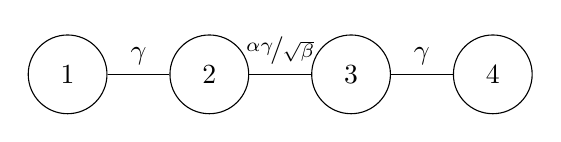
\begin{tikzpicture}[scale=0.9]
            % Draw nodes
            \node[circle, draw, fill=white, minimum size=1cm] (1) at (0,0) {1};
            \node[circle, draw, fill=white, minimum size=1cm] (2) at (2,0) {2};
            \node[circle, draw, fill=white, minimum size=1cm] (3) at (4,0) {3};
            \node[circle, draw, fill=white, minimum size=1cm] (4) at (6,0) {4};
            
            % Draw connections
            \draw[-] (1) -- (2) node[midway, above] {$\gamma$};
            \draw[-] (2) -- (3) node[midway, above] {$\nicefrac{\alpha\gamma}{\sqrt{\beta}}$};
            \draw[-] (3) -- (4) node[midway, above] {$\gamma$};
        \end{tikzpicture}
        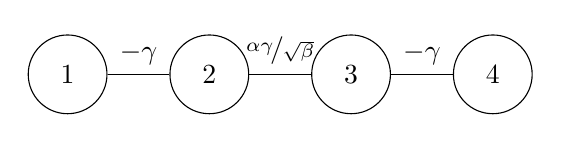
\begin{tikzpicture}[scale=0.9]
            % Draw nodes
            \node[circle, draw, fill=white, minimum size=1cm] (1) at (0,0) {1};
            \node[circle, draw, fill=white, minimum size=1cm] (2) at (2,0) {2};
            \node[circle, draw, fill=white, minimum size=1cm] (3) at (4,0) {3};
            \node[circle, draw, fill=white, minimum size=1cm] (4) at (6,0) {4};
            
            % Draw connections
            \draw[-] (1) -- (2) node[midway, above] {$-\gamma$};
            \draw[-] (2) -- (3) node[midway, above] {$\nicefrac{\alpha\gamma}{\sqrt{\beta}}$};
            \draw[-] (3) -- (4) node[midway, above] {$-\gamma$};
        \end{tikzpicture}
    \caption{\small The top diagram shows the edge weight configuration for the first step of the two-step PST protocol on the path graph P$_4$, while the bottom diagram represents the configuration for the second step. Note that the edge weights on the left and right have reversed polarity in the second step, i.e., $\gamma \rightarrow -\gamma$, and $\alpha,\beta,\gamma\in\mathbb{R}$.}
    \label{fig:p_4 two step}
\end{figure}

\paragraph{An unbounded family}
In the course of my investigation, I identified an unbounded family (Fig.~\ref{fig:p_4 two step}) that guarantees two-step perfect quantum state transfer in the P$_4$ chain from node 1 to node 4. The family is characterized by the following relations:
\begin{align}
    \label{eq:beta}
    \beta &= 7 + 8n = (5 + p)(3 - p + 8m), \\
    \alpha &= 2 + 2p - 8m, \\
    &\text{where} \quad 
    \begin{cases}
        n = 0,1,2,\dots, \\
        m = 0,1,2,\dots,n.
    \end{cases} \nonumber
\end{align}
Here, $p \in \mathbb{Z}$ is an integer parameter. For each solution, if the ratio $\nicefrac{\alpha}{\sqrt{\beta}}$ is in its simplest form $\nicefrac{\alpha'}{\sqrt{\beta'}}$ with $\alpha', \beta' \in \mathbb{Z}$, then the minimum time required to achieve perfect fidelity is given by:
\begin{equation}
    \tilde{t}= \tilde{t}' = \frac{\sqrt{\beta'} \pi}{4\gamma},
\end{equation}
where $\tilde{t}$ is the dimensionless runtime in the first step, and $\tilde{t}'$ is that in the second step.

To generate valid instances of this family, one first chooses any non-negative integer $n$, then selects an integer $m$ such that $0 \leq m \leq n$. Substituting $(n, m)$ into Eq.~\ref{eq:beta} yields a quadratic equation in $p$, which admits two solutions for $p$; however, only those integer values of $p$ correspond to valid two-step PST configurations. Once an eligible $p$ is found, the corresponding parameters $\alpha$ and $\beta$ can be evaluated explicitly. These determine the relative coupling strengths of the edges required to realize two-step PST from node 1 to node 4. Solutions for $n = 1$ through $9$ are provided in the table in Appendix C.

\paragraph{Formulation of the family: the magic number `4'}
The formulation of the P$_4$ two-step PST family equation was the result of a careful examination of the long list of irrational edge weight solutions generated by the optimizer (a highlight of the optimized solutions, with the repeating or invalid ones removed, can be found in Appendix B). At first glance, a recurring pattern was observed in a subset of solutions where the middle edge weight took the form $\nicefrac{6}{\sqrt{7}}$, $\nicefrac{22}{\sqrt{23}}$, $\nicefrac{30}{\sqrt{31}}$, and $\nicefrac{46}{\sqrt{47}}$. This suggested a tentative structure of the form $\nicefrac{(6 + 8n)}{\sqrt{7 + 8n}}$, where $n$ is a non-negative integer. However, several other solutions appeared to be exceptions to this rule, including values like $\nicefrac{10}{\sqrt{39}}$, $\nicefrac{6}{\sqrt{55}}$, $\nicefrac{2}{3\sqrt{7}}$, and $\nicefrac{2}{\sqrt{143}}$. Initially, these were regarded as outliers, lacking any clear connection to the earlier pattern.

A deeper analysis revealed that the denominators in all cases could be factorized into two positive integers such that one takes the form $(5 + r)$ and the other $(3 + s)$, where the sum $r + s$ is always a multiple of 8, i.e., $r + s = 8n$ for some non-negative integer $n$. Furthermore, the corresponding numerators consistently equal the difference between these two factors. That is, each middle edge weight can be written as the difference of the two factors divided by the square root of their product: $\nicefrac{(A - B)}{\sqrt{AB}}$, where $AB$ is the product forming the denominator, and $A$, $B$ are the two factors described above. This realization revealed that the earlier simple-looking solutions were, in fact, not special cases but members of the same unified structure.

An interesting observation is that within this family, any two edge weights that reduce to a fraction with the same square root in the denominator after simplification—i.e., having the same $\sqrt{\beta'}$ in their simplest form—share the exact same PST time, given by $t = \nicefrac{\sqrt{\beta'} \pi}{4\gamma}$.

Curiously, the number 4 appears multiple times in the formulation of this family. Not only does it arise in the denominator of the PST time expression, but it also matches the number of nodes in the path graph P$_4$. This led to a wild, perhaps naive, hypothesis: that this formulation might generalize to longer path graphs P$_n$, with similar structural rules governed by the graph’s size. If true, this would be a remarkable result—because in such a generalization, the larger the graph, the faster the transfer time, due to the $\nicefrac{1}{4\gamma}$ scaling being replaced by a possibly even smaller factor. This idea is highly speculative but extremely worth investigating.

\paragraph{Two-step PST revealed as one-step PST}
After studying numerous plots of the probability at node 4 as a function of time, a striking pattern emerged: the second step in the two-step PST protocol has no effect on the dynamics. Specifically, the probability amplitude at node 4 remains unchanged after the second step is applied (as shown in Fig.~\ref{fig:p4 (1)} and Fig.~\ref{fig:p4 (2)}). This indicates that the edge weight adjustments are effectively redundant in the P$_4$ chain. Furthermore, it was consistently observed that the second step always occurs at the peak of the probability distribution at node 4. These findings suggest that, for P$_4$, two-step PST is in fact equivalent to one-step PST. The newly discovered two-step PST family was independently verified using Mathematica simulations to also satisfy the criteria for one-step PST, confirming that this family simultaneously characterizes both one-step and two-step PST in P$_4$.

\begin{figure}
    \centering
    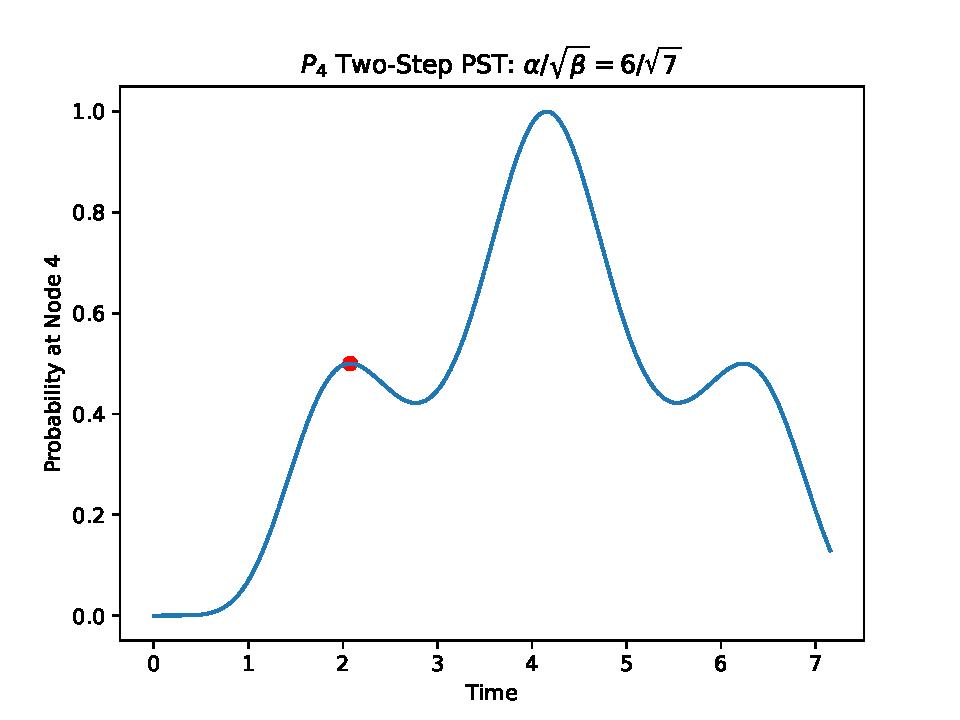
\includegraphics[width=0.49\textwidth]{p_4 (1).pdf}
    \caption{\small Probability of finding the walker at node 4 over time on the path graph P$_4$ with $\nicefrac{\alpha}{\beta}=\nicefrac{6}{\sqrt{7}}$, using a two-step quantum walk protocol. The red dot indicates the transition point where the second step begins, corresponding to a change in edge weights. An infidelity of $0$ is achieved at $\tilde{t} =\nicefrac{\sqrt{7}\pi}{2}$.}
    \label{fig:p4 (1)}
\end{figure}

\begin{figure}
    \centering
    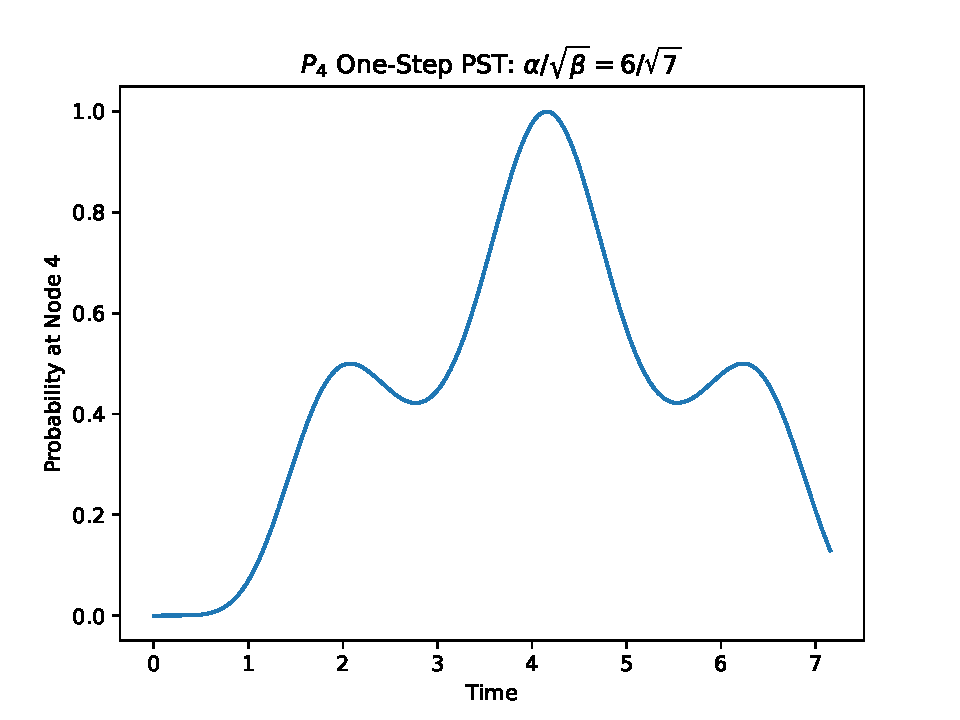
\includegraphics[width=0.49\textwidth]{p_4 (2).pdf}
    \caption{\small Probability of finding the walker at node 4 over time on the path graph P$_4$, without applying a second-step evolution. As in the two-step case (Fig.~\ref{fig:p4 (1)}), the system reaches an infidelity of $0$ at $\tilde{t} =\nicefrac{\sqrt{7}\pi}{2}$, indicating that PST can occur in a single step as well for this configuration.}
    \label{fig:p4 (2)}
\end{figure}

\subsection{C$_3$: Two-Step PST from Node 1 to Node 2}
In the case of the cycle graph C$_3$ (Fig.~\ref{fig:c3 node 1 to node 2}), an exact mathematical form underlying the observed irrational edge weight ratios could not be determined. The complexity of the values involved hindered any successful pattern recognition (a highlight of the optimized solutions can be found in Appendix B). However, several qualitative observations were made. Notably, the fidelity at node 2 reaches values extremely close to unity at specific runtimes, and these runtimes are frequently rational multiples of $\pi$. This behavior strongly suggests the presence of PST rather than PGST, as PST is commonly associated with transfer times involving $\pi$ as a factor. Further analysis of the probability amplitude at node 2 over time revealed that all cases studied could be achieved within a single step; examples can be found in Fig.~\ref{fig:c3 (1)} and Fig.~\ref{fig:c3 (2)}. This again confirms that, as in the P$_4$ case, what initially appears to be two-step PST in C$_3$ can in fact be fully realized within a single step. 

\begin{figure}
    \centering
    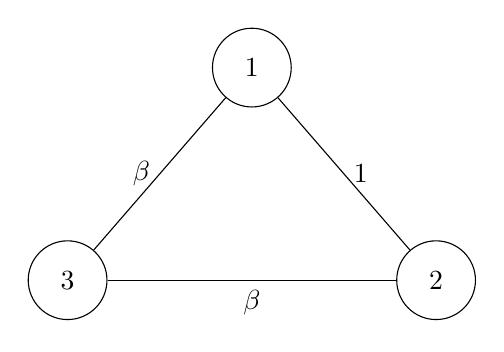
\begin{tikzpicture}[scale=0.9]
        % Draw nodes
        \node[circle, draw, fill=white, minimum size=1cm] (1) at (0,1.5) {1};
        \node[circle, draw, fill=white, minimum size=1cm] (2) at (2.6,-1.5) {2};
        \node[circle, draw, fill=white, minimum size=1cm] (3) at (-2.6,-1.5) {3};
        
        % Draw connections
        \draw[-] (1) -- (2) node[midway, right] {$1$};
        \draw[-] (2) -- (3) node[midway, below] {$\beta$};
        \draw[-] (3) -- (1) node[midway, left] {$\beta$};
        
        % Labels
        \node[below] at (1) {};
        \node[below] at (2) {};
        \node[below] at (3) {};
    \end{tikzpicture}
        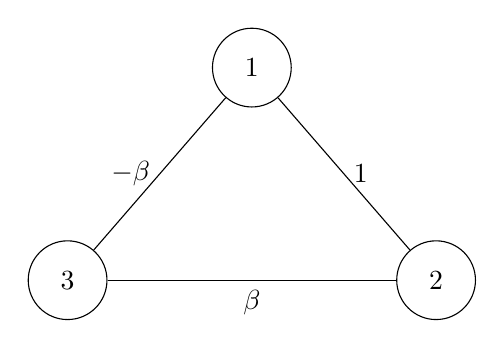
\begin{tikzpicture}[scale=0.9]
        % Draw nodes
        \node[circle, draw, fill=white, minimum size=1cm] (1) at (0,1.5) {1};
        \node[circle, draw, fill=white, minimum size=1cm] (2) at (2.6,-1.5) {2};
        \node[circle, draw, fill=white, minimum size=1cm] (3) at (-2.6,-1.5) {3};
        
        % Draw connections
        \draw[-] (1) -- (2) node[midway, right] {$1$};
        \draw[-] (2) -- (3) node[midway, below] {$\beta$};
        \draw[-] (3) -- (1) node[midway, left] {$-\beta$};
        
        % Labels
        \node[below] at (1) {};
        \node[below] at (2) {};
        \node[below] at (3) {};
    \end{tikzpicture}
    \caption{\small Two-step PST configuration on the cycle graph C$_3$ for transfer from node 1 to node 2 where $\beta\in\mathbb{R}$. The top diagram shows the edge weights during the first step, and the bottom diagram shows those used in the second step. The only change between steps is a sign flip on the edge between nodes 1 and 3, i.e., $ \beta \to -\beta $, while all other weights remain fixed.}
    \label{fig:c3 node 1 to node 2}
\end{figure}

\begin{figure}
    \centering
    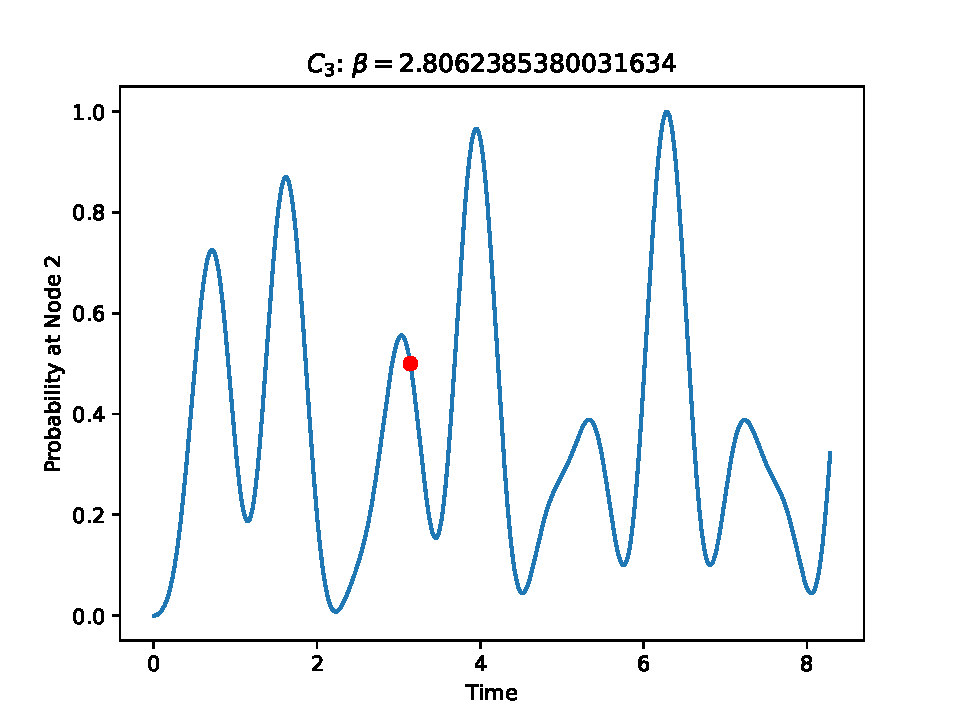
\includegraphics[width=0.49\textwidth]{c_3 (1).pdf}
    \caption{\small Probability of finding the walker at node 2 over time on the cycle graph C$_3$ with $\beta\approx2.81$, under a two-step PST protocol. The red dot marks the moment when the second step begins—that is, when the edge weights are adjusted to implement the second evolution. An infidelity below $10^{-12}$ is achieved at $\tilde{t} \approx 2\pi$.}
    \label{fig:c3 (1)}
\end{figure}

\begin{figure}
    \centering
    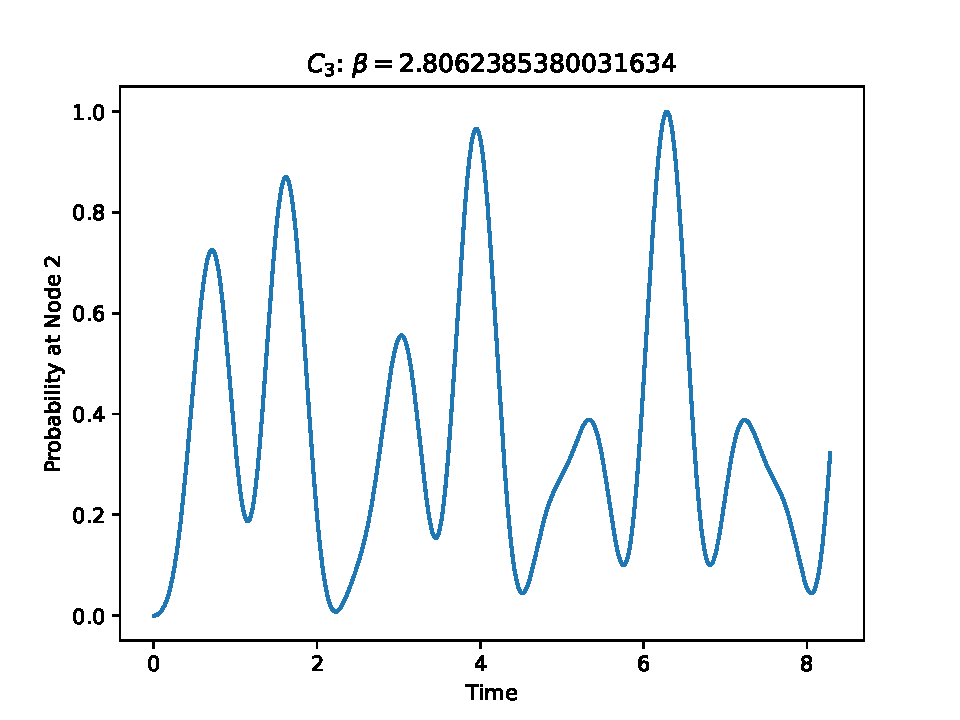
\includegraphics[width=0.49\textwidth]{c_3 (2).pdf}
    \caption{\small Probability of finding the walker at node 2 over time on the cycle graph C$_3$, without applying a second-step evolution. As in the two-step case (Fig.~\ref{fig:c3 (1)}), an infidelity below $10^{-12}$ is achieved at $\tilde{t} \approx 2\pi$, indicating the second step does not change the system dynamics at all.}
    \label{fig:c3 (2)}
\end{figure}

\subsection{C$_3$: Two-Step PST from Node 1 to Node 3}
This case marks the first instance where the second step is demonstrably necessary. Numerous asymmetric optimized configurations (Fig.~\ref{fig:c3 node 1 to node 3}) were discovered, and it was observed that, without applying the second step, the fidelity at node 3 oscillates as a periodic wave packet that never reaches unity — not even approximately (Fig.~\ref{fig:c3 (8)}). However, once the second step is applied, the fidelity sharply increases and approaches values extremely close to one shortly thereafter (Fig.~\ref{fig:c3 (7)}). Whether these cases correspond to PST or merely PGST, the result clearly demonstrates that the two-step PST framework has practical significance. In particular, it provides strong evidence that two-step PST is not only theoretically interesting but may also be essential for achieving perfect fidelity in certain asymmetric graphs where a one-step protocol fails.

\begin{figure}
    \centering
    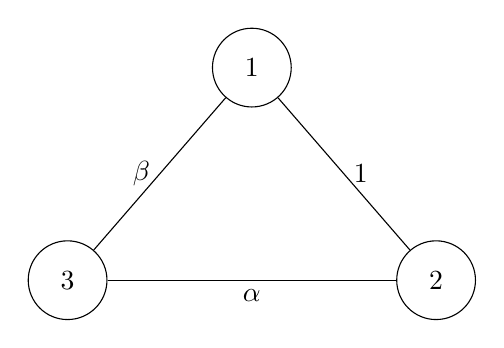
\begin{tikzpicture}[scale=0.9]
        % Draw nodes
        \node[circle, draw, fill=white, minimum size=1cm] (1) at (0,1.5) {1};
        \node[circle, draw, fill=white, minimum size=1cm] (2) at (2.6,-1.5) {2};
        \node[circle, draw, fill=white, minimum size=1cm] (3) at (-2.6,-1.5) {3};
        
        % Draw connections
        \draw[-] (1) -- (2) node[midway, right] {$1$};
        \draw[-] (2) -- (3) node[midway, below] {$\alpha$};
        \draw[-] (3) -- (1) node[midway, left] {$\beta$};
        
        % Labels
        \node[below] at (1) {};
        \node[below] at (2) {};
        \node[below] at (3) {};
    \end{tikzpicture}
        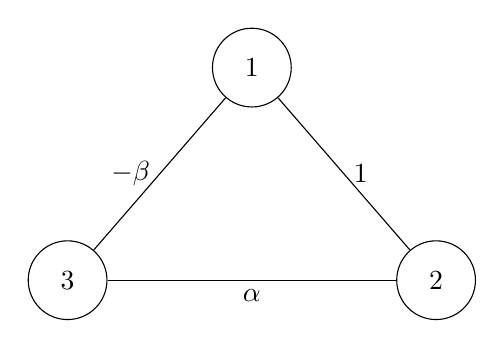
\begin{tikzpicture}[scale=0.9]
        % Draw nodes
        \node[circle, draw, fill=white, minimum size=1cm] (1) at (0,1.5) {1};
        \node[circle, draw, fill=white, minimum size=1cm] (2) at (2.6,-1.5) {2};
        \node[circle, draw, fill=white, minimum size=1cm] (3) at (-2.6,-1.5) {3};
        
        % Draw connections
        \draw[-] (1) -- (2) node[midway, right] {$1$};
        \draw[-] (2) -- (3) node[midway, below] {$\alpha$};
        \draw[-] (3) -- (1) node[midway, left] {$-\beta$};
        
        % Labels
        \node[below] at (1) {};
        \node[below] at (2) {};
        \node[below] at (3) {};
    \end{tikzpicture}
    \caption{\small Two-step PST configuration on the cycle graph C$_3$ where $\alpha,\beta\in\mathbb{R}$, for transfer from node 1 to node 3. The top diagram shows the edge weights during the first step, and the bottom diagram shows those used in the second step. The only change between steps is a sign flip on the edge between nodes 1 and 3, i.e., $ \beta \to -\beta $, while all other weights remain fixed.}
    \label{fig:c3 node 1 to node 3}
\end{figure}

\begin{figure}
    \centering
    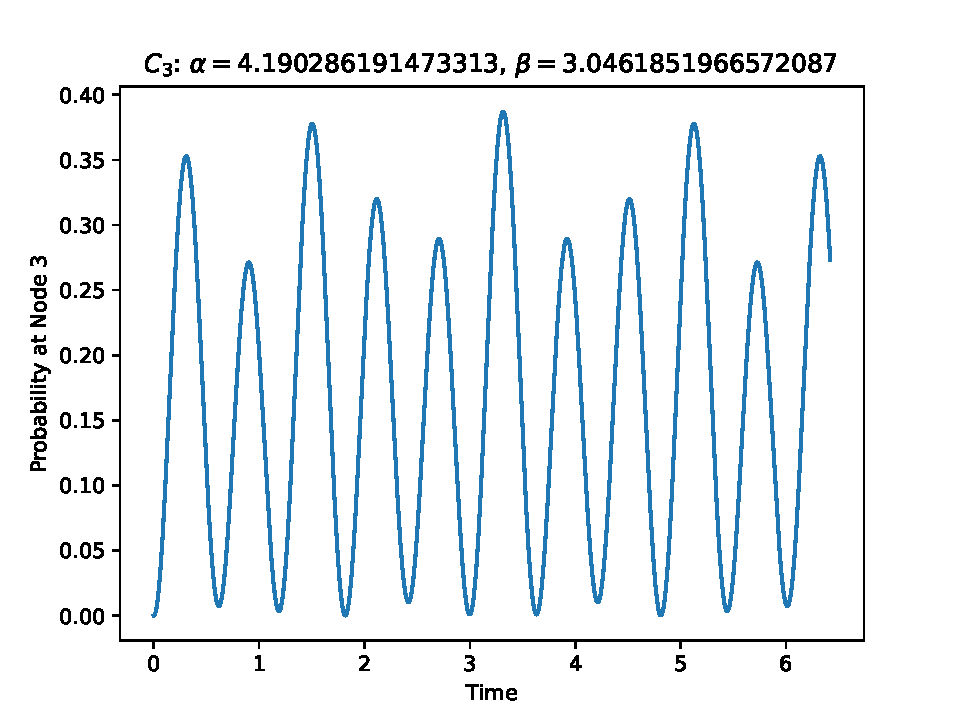
\includegraphics[width=0.49\textwidth]{c_3 (8).pdf}
    \caption{\small Probability of finding the walker at node 3 over time on the cycle graph C$_3$ with $\alpha\approx4.19$ and $\beta\approx3.05$, under a one-step evolution from node 1. The resulting wave packet is periodic and remains bounded below a probability of 0.5 throughout the evolution.}
    \label{fig:c3 (8)}
\end{figure}

\section{Conclusion}
This project investigated the phenomenon of two-step perfect quantum state transfer in continuous-time quantum walks on small graphs, with a particular focus on the path graph P$_4$ and the cycle graph C$_3$. Through the use of numerical optimization and analytical inspection, an unbounded family of two-step PST solutions was discovered for P$_4$, characterized by a not-so-elegant parameterization. Interestingly, this family was shown to also satisfy the conditions for one-step PST, as verified by Mathematica simulations. In this case, the second step had no influence on the state transfer fidelity, revealing that the underlying mechanism is fundamentally one-step in nature.
\begin{figure}
    \centering
    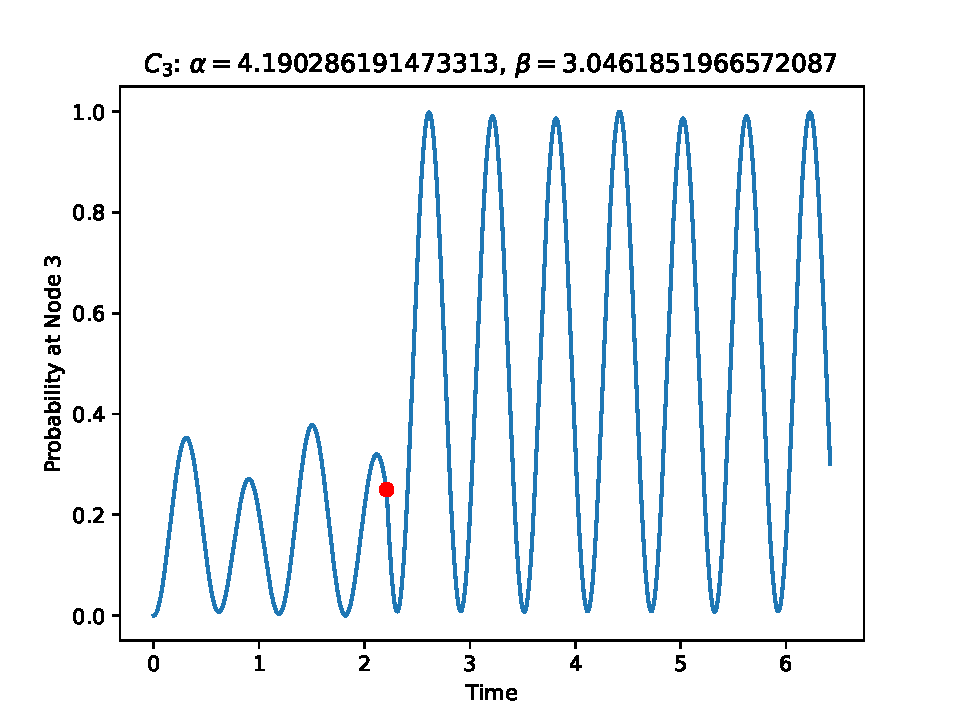
\includegraphics[width=0.49\textwidth]{c_3 (7).pdf}
    \caption{\small Probability of finding the walker at node 3 over time on the cycle graph C$_3$ with $\alpha\approx4.19$ and $\beta\approx3.05$, using a two-step protocol from node 1. The red dot indicates the moment when the second step begins, corresponding to a change in edge weights. An infidelity below $10^{-12}$ is achieved at $\tilde{t} \approx 4.42$.}
    \label{fig:c3 (7)}
\end{figure}

On the other hand, investigations on the cycle graph C$_3$ yielded mixed outcomes. For transfer from node 1 to node 2, no general pattern could be identified, but the solutions still exhibited properties very close to one-step PST, with fidelity peaks occurring at rational multiples of $\pi$. For transfer from node 1 to node 3, the second step played a critical and nontrivial role for the first time. Without it, the fidelity remained bounded below unity, forming periodic oscillations. When the second step was applied, the fidelity rapidly approached values extremely close to one. This constitutes the first clear demonstration that a two-step protocol can provide capabilities not achievable with a single step alone.

Together, these results affirm that two-step PST is not merely a theoretical curiosity but a potentially essential mechanism for achieving high-fidelity quantum communication—particularly in asymmetric or otherwise constrained graph structures. The work establishes both the feasibility and the value of further theoretical development in the study of two-step PST.

\section{Future Directions}
This investigation opens several promising avenues for future research. One major question is whether perfect quantum state transfer on path graphs P$_n$ can be described by a general mathematical rule, extending the unbounded family identified for P$_4$ to longer chains. Understanding the underlying structure in higher-order paths could reveal deeper symmetries or scaling laws governing PST in linear quantum networks.

Another compelling direction concerns the role of two-step PST in asymmetric systems. The case of node 1 to node 3 in C$_3$ provided the first concrete evidence that a two-step protocol can enable likely-perfect fidelity where one-step methods fail. This raises the possibility that two-step PST is not merely an artifact of small graphs but a fundamental mechanism for achieving perfect transfer in asymmetrically weighted systems. A systematic study across a variety of asymmetric graphs could test this hypothesis.

Finally, an open question remains whether introducing additional steps—such as three-step PST—might reveal new or broader families of PST solutions. If successful, this could provide a generalized framework for multi-step quantum walks that enable perfect transfer in otherwise inaccessible configurations. Exploring this multi-step regime may unlock a richer class of graph structures for robust quantum communication.

\FloatBarrier
\onecolumngrid
\clearpage
\appendix
\section{Analytical Sample Calculation for P$_2$}
\begin{center}
    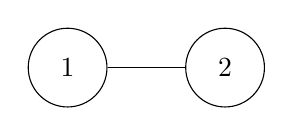
\begin{tikzpicture}
        \tikzstyle{every node}=[draw, circle, minimum size=10mm, inner sep=0pt]
        \node (A) at (0,0) {1};
        \node (B) at (2,0) {2};
        \draw (A) to (B);
    \end{tikzpicture}
    \captionof{figure}{\small Unweighted path graph P$_2$ consisting of two nodes connected by a single edge.}
\end{center}
The graph is represented by the Hamiltonian
\begin{equation}
    H=-J\begin{pmatrix}
        0&1\\
        1&0
    \end{pmatrix},
\end{equation}
where $J$ is a unit of energy and $-J$ relates the adjacency matrix to a Hermitian Hamiltonian.
This Hamiltonian indicates that the probability amplitude can `hop' between the two nodes.
The eigenvalues of $H$ are found to be:
\begin{align}
    \begin{vmatrix}
        -\lambda&-J\\
        -J&-\lambda
    \end{vmatrix}=&0,\nonumber\\
    \lambda^2-J^2=&0,\nonumber\\
    \lambda_1=J\;\;&\;\;\lambda_2=-J,
\end{align}
and their associated eigenvectors are
\begin{equation}
    u_1=\frac{1}{\sqrt{2}}\begin{pmatrix}
        1\\
        1
    \end{pmatrix}\quad u_2=\frac{1}{\sqrt{2}}\begin{pmatrix}
        1\\
        -1
    \end{pmatrix}.
\end{equation}
The time evolution of the quantum state is given by
\begin{equation}
    \label{eq:evolution}
    |\psi(t)\rangle=e^{-\nicefrac{iHt}{\hbar}}|\psi(0)\rangle.
\end{equation}
$H$ can be decomposed to
\begin{equation}
    \label{eq:hamiltonian spectral decomposition}
    H=\lambda_1|u_1\rangle\langle u_1|+\lambda_2|u_2\rangle\langle u_2|.
\end{equation}
By the approximation $e^x=\sum_{n=0}^\infty\nicefrac{x^n}{n!}$,
\begin{equation}
    \label{eq:exponential spectral decomposition}
    e^{-\nicefrac{iHt}{\hbar}}=e^{-\nicefrac{i\lambda_1t}{\hbar}}|u_1\rangle\langle u_1|+e^{-\nicefrac{i\lambda_2t}{\hbar}}|u_2\rangle\langle u_2|.
\end{equation}
To solve for $t$ in Eq.~\ref{eq:evolution}, $|\psi(0)\rangle$ and $|\psi(t)\rangle$ are needed. Assuming that the initial state is localised on node 1,
\begin{equation}
    \label{eq:initial state}
    |\psi(0)\rangle=\begin{pmatrix}
        1\\
        0
    \end{pmatrix}.
\end{equation}
For a perfect quantum state transfer, the final state should be localised on node 2, so
\begin{equation}
    \label{eq:final state}
    |\psi(t)\rangle=\begin{pmatrix}
        0\\
        1
    \end{pmatrix}.
\end{equation}
Putting Eq.~\ref{eq:exponential spectral decomposition}, Eq.~\ref{eq:initial state} and Eq.~\ref{eq:final state} into Eq.~\ref{eq:evolution},
\begin{align}
    \begin{pmatrix}
        0\\
        1
    \end{pmatrix}=&\left(e^{-\nicefrac{i\lambda_1t}{\hbar}}|u_1\rangle\langle u_1|+e^{-\nicefrac{i\lambda_2t}{\hbar}}|u_2\rangle\langle u_2|\right)\begin{pmatrix}
        1\\
        0
    \end{pmatrix},\nonumber\\
    \begin{pmatrix}
        0\\
        1
    \end{pmatrix}=&\begin{pmatrix}
        \nicefrac{e^{-\nicefrac{iJt}{\hbar}}+e^{\nicefrac{iJt}{\hbar}}}{2}&\nicefrac{e^{-\nicefrac{iJt}{\hbar}}-e^{\nicefrac{iJt}{\hbar}}}{2}\\
        \nicefrac{e^{-\nicefrac{iJt}{\hbar}}-e^{\nicefrac{iJt}{\hbar}}}{2}&\nicefrac{e^{-\nicefrac{iJt}{\hbar}}+e^{\nicefrac{iJt}{\hbar}}}{2}
    \end{pmatrix}\begin{pmatrix}
        1\\
        0
    \end{pmatrix},\nonumber\\
    \begin{pmatrix}
        0\\
        1
    \end{pmatrix}=&\begin{pmatrix}
        \cos{\frac{Jt}{\hbar}}\\
        -i\sin{\frac{Jt}{\hbar}}
    \end{pmatrix},
\end{align}
and $t$ is found to be $\nicefrac{\pi\hbar}{2J}$. In other words, the quantum state at node $1$ is transferred to node $2$ with perfect fidelity after $\nicefrac{\pi\hbar}{2J}$ seconds. To make it dimensionless, we can define the dimensionless time as $t=a\Tilde{t}$ where $a=\nicefrac{\hbar}{J}$. The dimensionless time $\Tilde{t}$ in this case is found to be
\begin{equation}
    \Tilde{t}=\frac{\pi}{2}.
\end{equation}
\section{Optimized Variables}
\begin{center}
    \begin{tabular}{||c c||} 
        \multicolumn{2}{c}{P$_4$ Node 1 to Node 4: Fidelity $>$ 0.999999999}\\
        \hline
        Edge Weights (Before): $[w_1,w_2,w_3]$&$t=t'$\\
        \hline
        [1.0, -8.775678756720122, 1.0]&6.982671079\\

        [1.0, -8.775692480914591, 1.0]&6.978872379\\

        [1.0, -8.775692507093504, 1.0]&6.978872542\\
        \hline
        [1.0, -9.220175551480535, 1.0]&7.323852643\\
        
        [1.0, -9.220160041813735, 1.0]&7.327560054\\
        \hline
        [1.0, -9.644230191589418, 1.0]&7.653361319\\
        \hline
        [1.0, -1.4363696430269532, 1.0]&7.659804294\\

        [1.0, -1.4363701167830498, 1.0]&7.650430304\\
        \hline
        [1.0, 10.050348592504676, 1.0]&7.97269521\\
        \hline
        [1.0, -10.440748415133244, 1.0]&8.272939815\\
        \hline
        [1.0, -3.227133528574531, 1.0]&8.274232835\\

        [1.0, -3.2271369323243624, 1.0]&8.277812482\\
        \hline
        [1.0, 0.16724843366067466, 1.0]&9.378249982\\
        \hline
        [1.0, 3.9652583074360974, 1.0]&9.900671203\\
        
        [1.0, -3.96525830774512, 1.0]&9.900670429\\
        \hline
        [1.0, -4.287482925652273, 1.0]&10.6273849\\
        \hline 
    \end{tabular}
    \captionof{table}{Edge weights and corresponding times $t = t'$ for the path from Node 1 to Node 4 in the P$_4$ graph, with fidelity exceeding 0.999999999. The table lists the edge weights before transformation in the form $[w_1,w_2,w_3]$. After transformation, the edge weights become $[-w_1,w_2,-w_3]$.}
\end{center}
\begin{center}
    \begin{tabular}{||c c||}
        \multicolumn{2}{c}{P$_4$ Node 1 to Node 4: Fidelity $>$ 0.999999999 (Continued)}\\
        \hline
        Edge Weights (Before): $[w_1,w_2,w_3]$&$t=t'$\\
        \hline
        [1.0, 2.2677864162435357, 1.0]&2.081701141\\

        [1.0, 2.2677872585089562, 1.0]&2.0742356524309\\

        [1.0, -2.267787257589282, 1.0]&2.074246026\\

        [1.0, -2.267786417033427, 1.0]&2.08170109\\
        \hline
        [1.0, 0.5163978486429714, 1.0]&3.034013229\\
        
        [1.0, -0.5163973327358463, 1.0]&3.044563193\\

        [1.0, -0.5163978486459277, 1.0]&3.03401323\\
        \hline
        [1.0, 3.614820251255397, 1.0]&3.04014415\\
        
        [1.0, -3.614785401654898, 1.0]&3.03887772\\

        [1.0, -3.6147854023235837, 1.0]&3.038877381\\
        \hline
        [1.0, -4.587318653298133, 1.0]&3.764012455\\
        
        [1.0, -4.587316594892395, 1.0]&11.30253673\\

        [1.0, 4.587345143460048, 1.0]&3.767587833\\
        \hline
        [1.0, 5.388161262251575, 1.0]&4.370490101\\

        [1.0, -5.388204386530768, 1.0]&4.371473889\\
        \hline
        [1.0, -1.6012814463605203, 1.0]&4.909252167\\

        [1.0, -1.6012814463922922, 1.0]&4.909252043\\

        [1.0, -1.6012816295409682, 1.0]&4.9003682\\
        \hline
        [1.0, 6.084872739875749, 1.0]&4.902530395\\

        [1.0, -6.084866925228957, 1.0]&4.907089391\\

        [1.0, -6.084866943257897, 1.0]&4.907089902\\
        \hline
        [1.0, -6.709793237392034, 1.0]&5.382247619\\

        [1.0, -6.709793238127481, 1.0]&5.382247074\\

        [1.0, -6.709785918264255, 1.0]&5.386588214\\
        \hline
        [1.0, 0.809039874164738, 1.0]&5.818418956\\

        [1.0, 0.8090386679103602, 1.0]&5.824430125\\

        [1.0, -0.8090398741444761, 1.0]&5.818420127\\
        \hline
        [1.0, -7.281369869968289, 1.0]&5.822991142\\

        [1.0, -7.2813540562574275, 1.0]&5.826753211\\

        [1.0, -7.2813541158043575, 1.0]&5.826752993\\
        \hline
        [1.0, -0.2519763555275555, 1.0]&6.222707537\\
        \hline
        [1.0, 7.81127097891731, 1.0]&6.231891388\\

        [1.0, -7.811218900466319, 1.0]&6.235755067\\

        [1.0, -7.811260571812177, 1.0]&6.235917089\\
        \hline
        [1.0, -8.307465564796429, 1.0]&6.619834791\\

        [1.0, -8.307477689698592, 1.0]&6.615930995\\
        \hline
    \end{tabular}
    \captionof{table}{Continuation of TABLE I; edge weights and corresponding times $t = t'$ for the path from Node 1 to Node 4 in the P$_4$ graph, with fidelity exceeding 0.999999999. The table lists the edge weights before transformation in the form $[w_1,w_2,w_3]$. After transformation, the edge weights become $[-w_1,w_2,-w_3]$.}
\end{center}
\begin{center}
    \begin{tabular}{||c c||}
        \multicolumn{2}{c}{P$_4$ Node 1 to Node 4: Fidelity $>$ 0.999999999999}\\
        \hline
        Edge Weights (Before): $[w_1,w_2,w_3]$&$t=t'$\\
        \hline
        [1.0, -2.267786840422201, 1.0]&2.077304562\\

        [1.0, -2.267786840422201, 1.0]&2.077304562\\

        [1.0, -2.267786840422201, 1.0]&2.077304562\\
        \hline
        [1.0, 3.6147844511476226, 1.0]&3.042359822\\

        [1.0, 3.6147844511476226, 1.0]&3.042359822\\
        \hline
        [1.0, 4.587317100652229, 1.0]&3.767103882\\
        \hline
        [1.0, 0.5163977791040121, 1.0]&3.043224841\\
        
        [1.0, 0.5163979082935659, 1.0]&3.041398719\\
        \hline
        [1.0, -5.388159048452486, 1.0]&4.373342537\\

        [1.0, -5.388159073147655, 1.0]&4.37248137\\
        \hline
        [1.0, 1.6012815385662786, 1.0]&4.904019911\\
        \hline
        [1.0, 0.8090399266807671, 1.0]&5.823707582\\

        [1.0, 0.8090398347456658, 1.0]&5.825780094\\

        [1.0, 0.8090398347456658, 1.0]&5.825780094\\
        \hline
        [1.0, 6.709789588696451, 1.0]&5.384804545\\
        \hline
        [1.0, -0.2519763151128192, 1.0]&6.235895717\\
        \hline
    \end{tabular}
    \captionof{table}{Edge weights and corresponding times $t = t'$ for the path from Node 1 to Node 4 in the P$_4$ graph, with fidelity exceeding 0.999999999999. The table lists the edge weights before transformation in the form $[w_1,w_2,w_3]$. After transformation, the edge weights become $[-w_1,w_2,-w_3]$.}
\end{center}
\begin{center}
    \begin{tabular}{||c c||}
        \multicolumn{2}{c}{P$_4$ Node 1 to Node 4: Fidelity $>$ 0.999999999999999}\\
        \hline
        Edge Weights (Before): $[w_1 \; w_2 \; w_3]$&$t=t'$\\
        \hline
        [1.0, -2.2677868380760757, 1.0]&2.077831382\\

        [1.0, -2.2677868380760757, 1.0]&2.077831382\\
        \hline
        [1.0, -7.281358514018219, 1.0]&5.824775131\\
        \hline
        [1.0, 0.1672484025560938, 1.0]&9.392512825\\
        \hline
    \end{tabular}
    \captionof{table}{Edge weights and corresponding times $t = t'$ for the path from Node 1 to Node 4 in the P$_4$ graph, with fidelity exceeding 0.999999999999. The table lists the edge weights before transformation in the form $[w_1,w_2,w_3]$. After transformation, the edge weights become $[-w_1,w_2,-w_3]$.}
\end{center}
\begin{center}
    \begin{tabular}{||c c||}
        \multicolumn{2}{c}{C$_3$ Node 1 to Node 2: Fidelity $>$ 0.999999999}\\
        \hline
        Edge Weights (Before): $[w_1 \; w_2 \; w_3]$&$t=t'$\\
        \hline
        [1.0, 2.0916488556893857, 2.091614476453943]&1.047209413\\

        [1.0, 2.0917515812943277, 2.0916415560119344]&1.047185748\\

        [1.0, 2.091615661219744, 2.091716477549027]&1.047187637\\
        \hline
        [1.0, 4.227542432731449, 4.228295065841354]&1.047194318\\

        [1.0, 4.227538157532992, 4.22829227614664]&1.047195133\\

        [1.0, 4.227536004550318, 4.228289287140113]&1.047195662\\
        \hline
        [1.0, 5.64541775078533, 5.646164349155414]&3.141587739\\
        \hline
        [1.0, 1.369309304509472, 1.3692909635456583]&3.141634575\\
        \hline
        [1.0, 6.3541518473873095, 6.354143536884679]&1.047230273\\

        [1.0, 6.355041232947497, 6.353281446657205]&1.047196328\\

        [1.0, 6.3532249320447605, 6.3549835838974795]&1.047198668\\
        \hline
        [1.0, 0.6123972894962187, 0.6123745624670441]&3.141584849\\
        \hline
        [1.0, 3.518055948672872, 3.5175491236546765]&3.14159454\\

        [1.0, 3.5175673763293944, 3.518075365770143]&3.141590556\\
        \hline
        [1.0, 2.8064066043074347, 2.8060994691493977]&3.141589673\\
        \hline
        [1.0, 0.4922986614010462, 0.492266407009438]&7.330391805\\
        \hline
        [1.0, 4.936592240678165, 4.937635439362065]&3.141591194\\
        \hline
    \end{tabular}
    \captionof{table}{Edge weights and corresponding times $t = t'$ for the path from Node 1 to Node 2 in the C$_3$ graph, with fidelity exceeding 0.999999999. The table lists the edge weights before transformation in the form $[w_1,w_2,w_3]$. After transformation, the edge weights become $[w_1,-w_2,w_3]$.}
\end{center}
\begin{center}
    \begin{tabular}{||c c||}
        \multicolumn{2}{c}{C$_3$ Node 1 to Node 2: Fidelity $>$ 0.999999999999}\\
        \hline
        Edge Weights (Before): $[w_1 \; w_2 \; w_3]$&$t=t'$\\
        \hline
        [1.0, 4.227894604123888, 4.2278708639953315]&1.047197605\\

        [1.0, 4.227894358428255, 4.227870601304786]&1.047197663\\

        [1.0, 4.2278727436079935, 4.227896567879388]&1.047197469\\
        \hline
        [1.0, 2.0916504914527674, 2.0916518974342933]&1.047197221\\

        [1.0, 2.091646427600161, 2.0916508183940046]&1.047197826\\

        [1.0, 2.091647603070719, 2.091650822524275]&1.047196924\\
        \hline
        [1.0, 3.5178195270160675, 3.51780347526475]&3.141592733\\

        [1.0, 3.517804097863254, 3.517820172580133]&3.141592577\\

        [1.0, 3.5178195148023295, 3.5178035092298523]&3.141592725\\
        \hline
        [1.0, 6.354103832062821, 6.354159432824193]&1.047197585\\
        \hline
        [1.0, 2.8062481729441497, 2.8062385387190467]&3.141592558\\
        \hline
        [1.0, 0.23452109465991697, 0.23452208917607806]&5.235986388\\
        \hline
        [1.0, 6.354161192366017, 6.3541055655312855]&1.04719752\\
        \hline
    \end{tabular}
    \captionof{table}{Edge weights and corresponding times $t = t'$ for the path from Node 1 to Node 2 in the C$_3$ graph, with fidelity exceeding 0.999999999999. The table lists the edge weights before transformation in the form $[w_1,w_2,w_3]$. After transformation, the edge weights become $[w_1,-w_2,w_3]$.}
\end{center}
\begin{center}
    \begin{tabular}{||c c||}
        \multicolumn{2}{c}{C$_3$ Node 1 to Node 3: Fidelity $>$ 0.999999999}\\
        \hline
        Edge Weights (Before): $[w_1 \; w_2 \; w_3]$&$t=t'$\\
        \hline
        [1.0, 1.0000627779323967, 2.031426058335637]&3.608501622\\

        [1.0, 1.0000669533549078, 2.0314323082702863]&3.60849027\\

        [1.0, 1.0000667664681648, 2.0314318871757537]&3.608491026\\
        \hline
        [1.0, 1.0001094131525905, 2.8383986986304652]&6.271967381\\
        \hline
        [1.0, 0.9999915036797877, 1.296416251389392]&4.038829705\\
        \hline
        [1.0, 1.0001342865757132, 4.264250107353341]&3.683711795\\

        [1.0, 1.0001274936176199, 4.264640545001713]&1.227785759\\

        [1.0, 1.0001495644623593, 4.264277174537256]&3.683628415\\
        \hline
        [1.0, 1.0000672571444604, 0.4781038628347857]&2.190311489\\

        [1.0, 1.0000678911717877, 0.4781034622718982]&2.190313873\\

        [1.0, 1.0000668024069261, 0.4781037273251023]&2.190312091\\
        \hline
        [1.0, 0.999999129841404, 1.6329609390345385]&1.923849528\\

        [1.0, 0.9999911949594547, 1.6330045239292843]&1.923822082\\
        \hline
        [1.0, 1.0001168600232988, 3.2072873608895]&2.938548708\\

        [1.0, 1.000118226943861, 3.2072874825407336]&2.938548369\\
        \hline
        [1.0, 1.000177767159788, 0.23654767723475098]&4.427013769\\
        \hline
    \end{tabular}
    \captionof{table}{Edge weights and corresponding times $t = t'$ for the path from Node 1 to Node 3 in the C$_3$ graph, with fidelity exceeding 0.999999999. The table lists the edge weights before transformation in the form $[w_1,w_2,w_3]$. After transformation, the edge weights become $[w_1,-w_2,w_3]$.}
\end{center}
\begin{center}
    \begin{tabular}{||c c||}
        \multicolumn{2}{c}{C$_3$ Node 1 to Node 3: Fidelity $>$ 0.999999999999}\\
        \hline
        Edge Weights (Before): $[w_1 \; w_2 \; w_3]$&$t=t'$\\
        \hline
        [1.0, 1.0000056271301678, 0.23652567775072858]&4.427416364\\
        \hline
        [1.0, 1.000002106021208, 2.031336609147502]&3.60865035\\

        [1.0, 1.0000021099917753, 2.0313366140010753]&3.608650341\\

        [1.0, 1.0000021077237324, 2.031336611826904]&3.60865034\\
        \hline
        [1.0, 0.9999978618377054, 0.47809105049509043]&2.190372718\\

        [1.0, 1.000002140357264, 0.47809183515441567]&2.190368954\\
        \hline
        [1.0, 1.0000004129507405, 1.2964078289722214]&4.038843198\\
        \hline
        [1.0, 1.0000004683087362, 1.632994261899121]&1.923823681\\

        [1.0, 0.9999995121710327, 1.6329920882824183]&1.923825793\\

        [1.0, 0.9999999821830493, 1.6329920402749796]&1.923825518\\
        \hline
        [1.0, 1.0000037241144935, 3.20713969861044]&2.938686386\\
        \hline
    \end{tabular}
    \captionof{table}{Edge weights and corresponding times $t = t'$ for the path from Node 1 to Node 3 in the C$_3$ graph, with fidelity exceeding 0.999999999999. The table lists the edge weights before transformation in the form $[w_1,w_2,w_3]$. After transformation, the edge weights become $[w_1,-w_2,w_3]$.}
\end{center}
\begin{center}
    \begin{tabular}{||c c||}
        \multicolumn{2}{c}{C$_3$ Node 1 to Node 3: Fidelity $>$ 0.999999999}\\
        \hline
        Edge Weights (Before): $[w_1 \; w_2 \; w_3]$&$t=t'$\\
        \hline
        [1.0, 4.966668010139432, 3.5824101220603324]&2.213370938\\
        \hline
        [1.0, 2.626107662589982, 1.9870253129406752]&2.19415966\\

        [1.0, 2.626019153056227, 1.9869249483426332]&2.194211858\\
        \hline
        [1.0, 3.019388275770154, 2.249123071255105]&4.400760107\\

        [1.0, 3.0194099539592303, 2.2491258982020446]&4.400742356\\
        \hline
        [1.0, 1.8296080121756138, 1.4743588551271927]&2.16994866\\

        [1.0, 1.8296188185217954, 1.4743703261290761]&2.169908176\\

        [1.0, 1.8295744499799356, 1.4743567317036832]&2.169934767\\
        \hline
        [1.0, 6.514908869965452, 4.660636426543189]&2.216720165\\

        [1.0, 6.514912275744246, 4.660633424425117]&2.216719864\\
        \hline
        [1.0, 4.190375519828131, 3.04627311787354]&2.210103095\\

        [1.0, 4.190372116427484, 3.0462740472577168]&2.21010433\\

        [1.0, 4.190320442978032, 3.04626247305939]&4.420247655\\
        \hline
        [1.0, 8.831622946956266, 6.284745496566233]&2.218877249\\

        [1.0, 8.831621549484437, 6.2847482033702]&2.218877111\\
        \hline
        [1.0, 4.9666694857153235, 3.582410192032633]&2.213370389\\

        [1.0, 4.9668665750817, 3.5826179453607008]&2.213272343\\

        [1.0, 4.966806828558542, 3.5826025794627467]&4.426584588\\
        \hline
    \end{tabular}
    \captionof{table}{Edge weights and corresponding times $t = t'$ for the path from Node 1 to Node 3 in the C$_3$ graph, with fidelity exceeding 0.999999999. The table lists the edge weights before transformation in the form $[w_1,w_2,w_3]$. After transformation, the edge weights become $[w_1,w_2,-w_3]$.}
\end{center}
\begin{center}
    \begin{tabular}{||c c||}
        \multicolumn{2}{c}{C$_3$ Node 1 to Node 3: Fidelity $>$ 0.999999999999}\\
        \hline
        Edge Weights (Before): $[w_1 \; w_2 \; w_3]$&$t=t'$\\
        \hline

        [1.0, 1.829576796794524, 1.4743389704963579]&2.169949868\\

        [1.0, 1.829576822324173, 1.4743392162611422]&2.169949501\\
        \hline
        [1.0, 6.515031592899615, 4.66077312237574]&2.216671657\\
        \hline
        [1.0, 4.190286191473313, 3.0461851966572087]&2.210153548\\

        [1.0, 4.190291562190012, 3.046190572715612]&2.210150502\\

        [1.0, 4.190289803246081, 3.0461902989145426]&4.420302312\\
        \hline
        [1.0, 1.4218099169058493, 1.2291346399776408]&4.288203328\\

        [1.0, 1.4218091270772508, 1.2291342647844747]&4.288204589\\
        \hline
        [1.0, 2.6260527751986107, 1.9869771197637223]&2.19420324\\
        \hline
        [1.0, 1.829576767196629, 1.4743388038769978]&2.169949821\\

        [1.0, 1.8295769040517138, 1.4743390872004336]&2.16994957\\
        \hline
        [1.0, 4.966767805859688, 3.5825097108373787]&4.426644629\\
        \hline
        [1.0, 7.287800965791545, 5.2015386755525235]&2.217618092\\
        \hline
        [1.0, 2.6260527073545514, 1.986977127650279]&2.194203306\\

        [1.0, 2.626052765144188, 1.986977158010557]&2.194203239\\
        \hline
    \end{tabular}
    \captionof{table}{Edge weights and corresponding times $t = t'$ for the path from Node 1 to Node 3 in the C$_3$ graph, with fidelity exceeding 0.999999999999. The table lists the edge weights before transformation in the form $[w_1,w_2,w_3]$. After transformation, the edge weights become $[w_1,w_2,-w_3]$.}
\end{center}
\section{P$_4$ PST from Node 1 to Node 4}
\begin{center}
    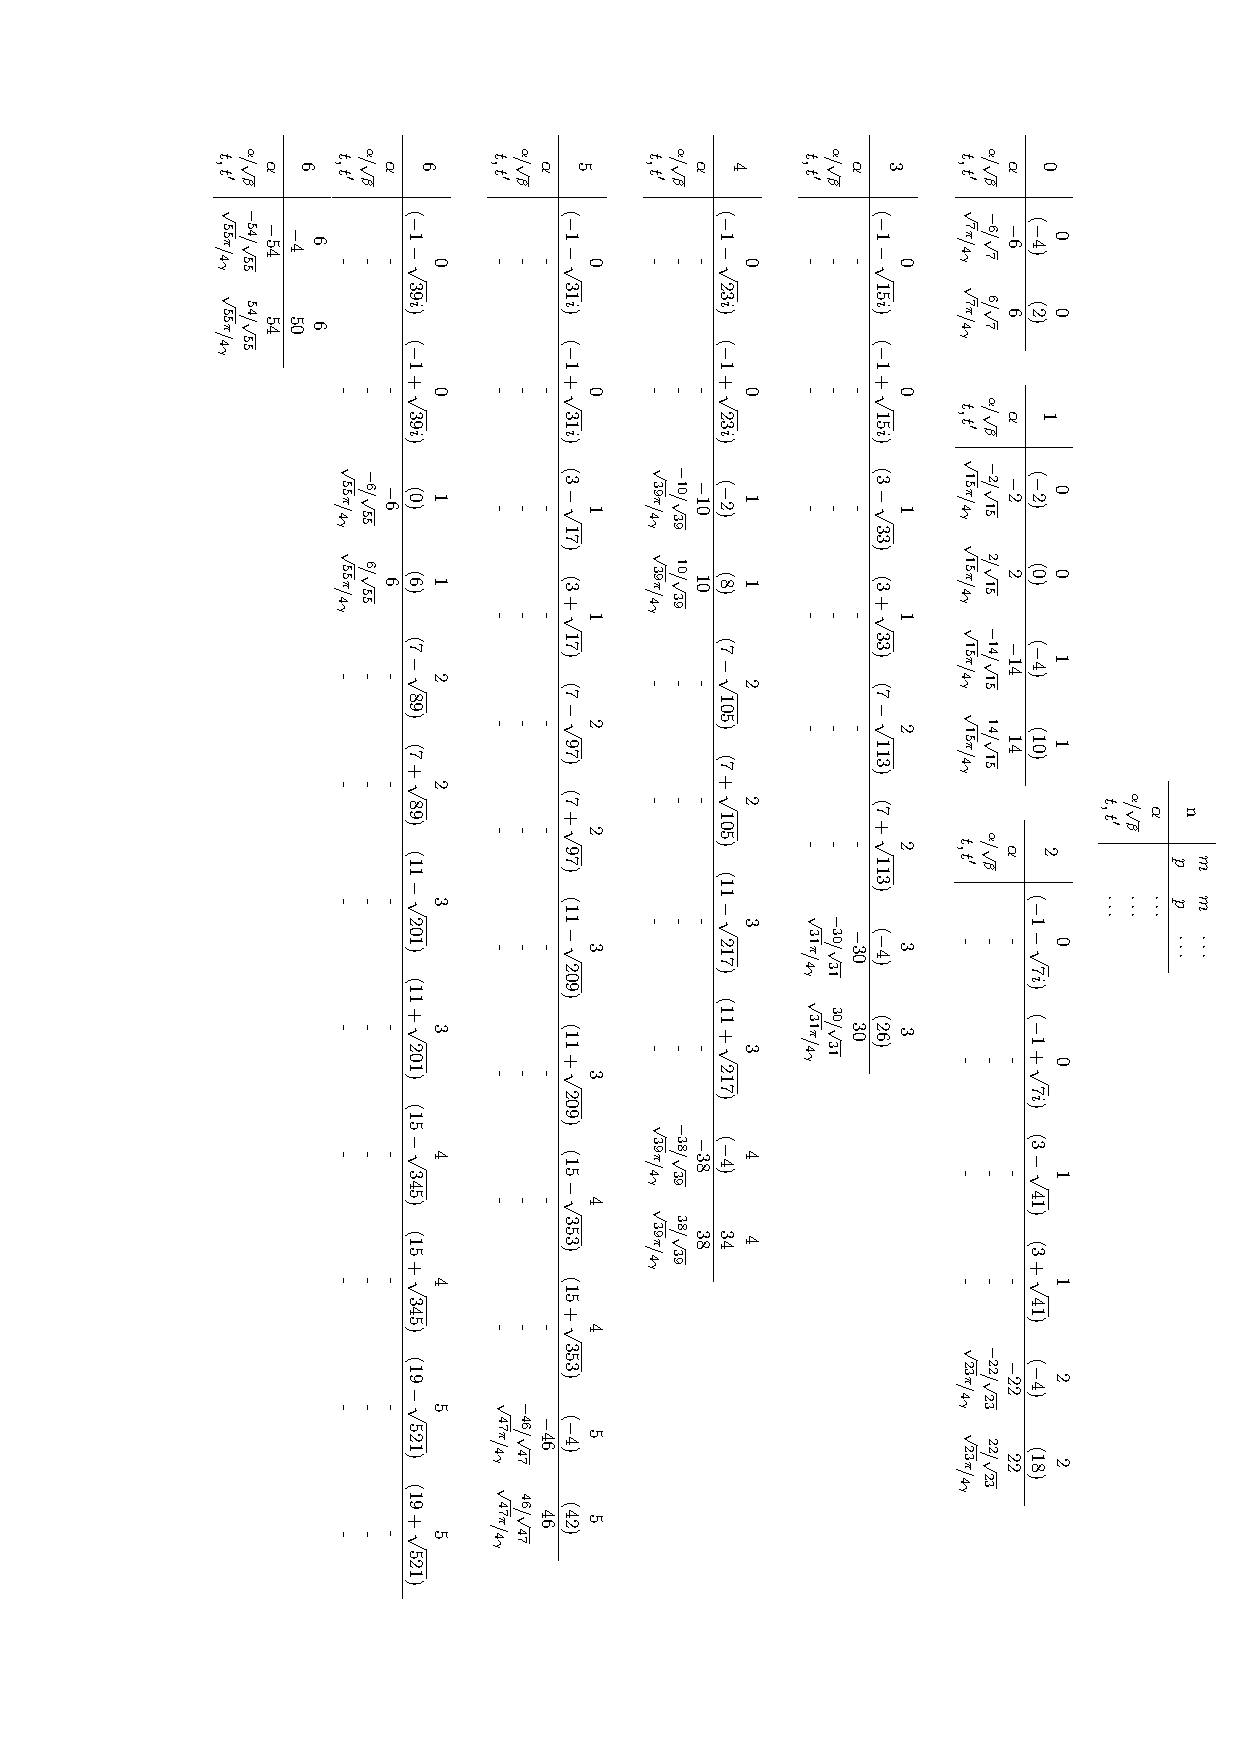
\includegraphics[width=\textwidth]{P4_PST_Node_1_to_Node_4 (1).pdf}
\end{center}
\begin{center}
    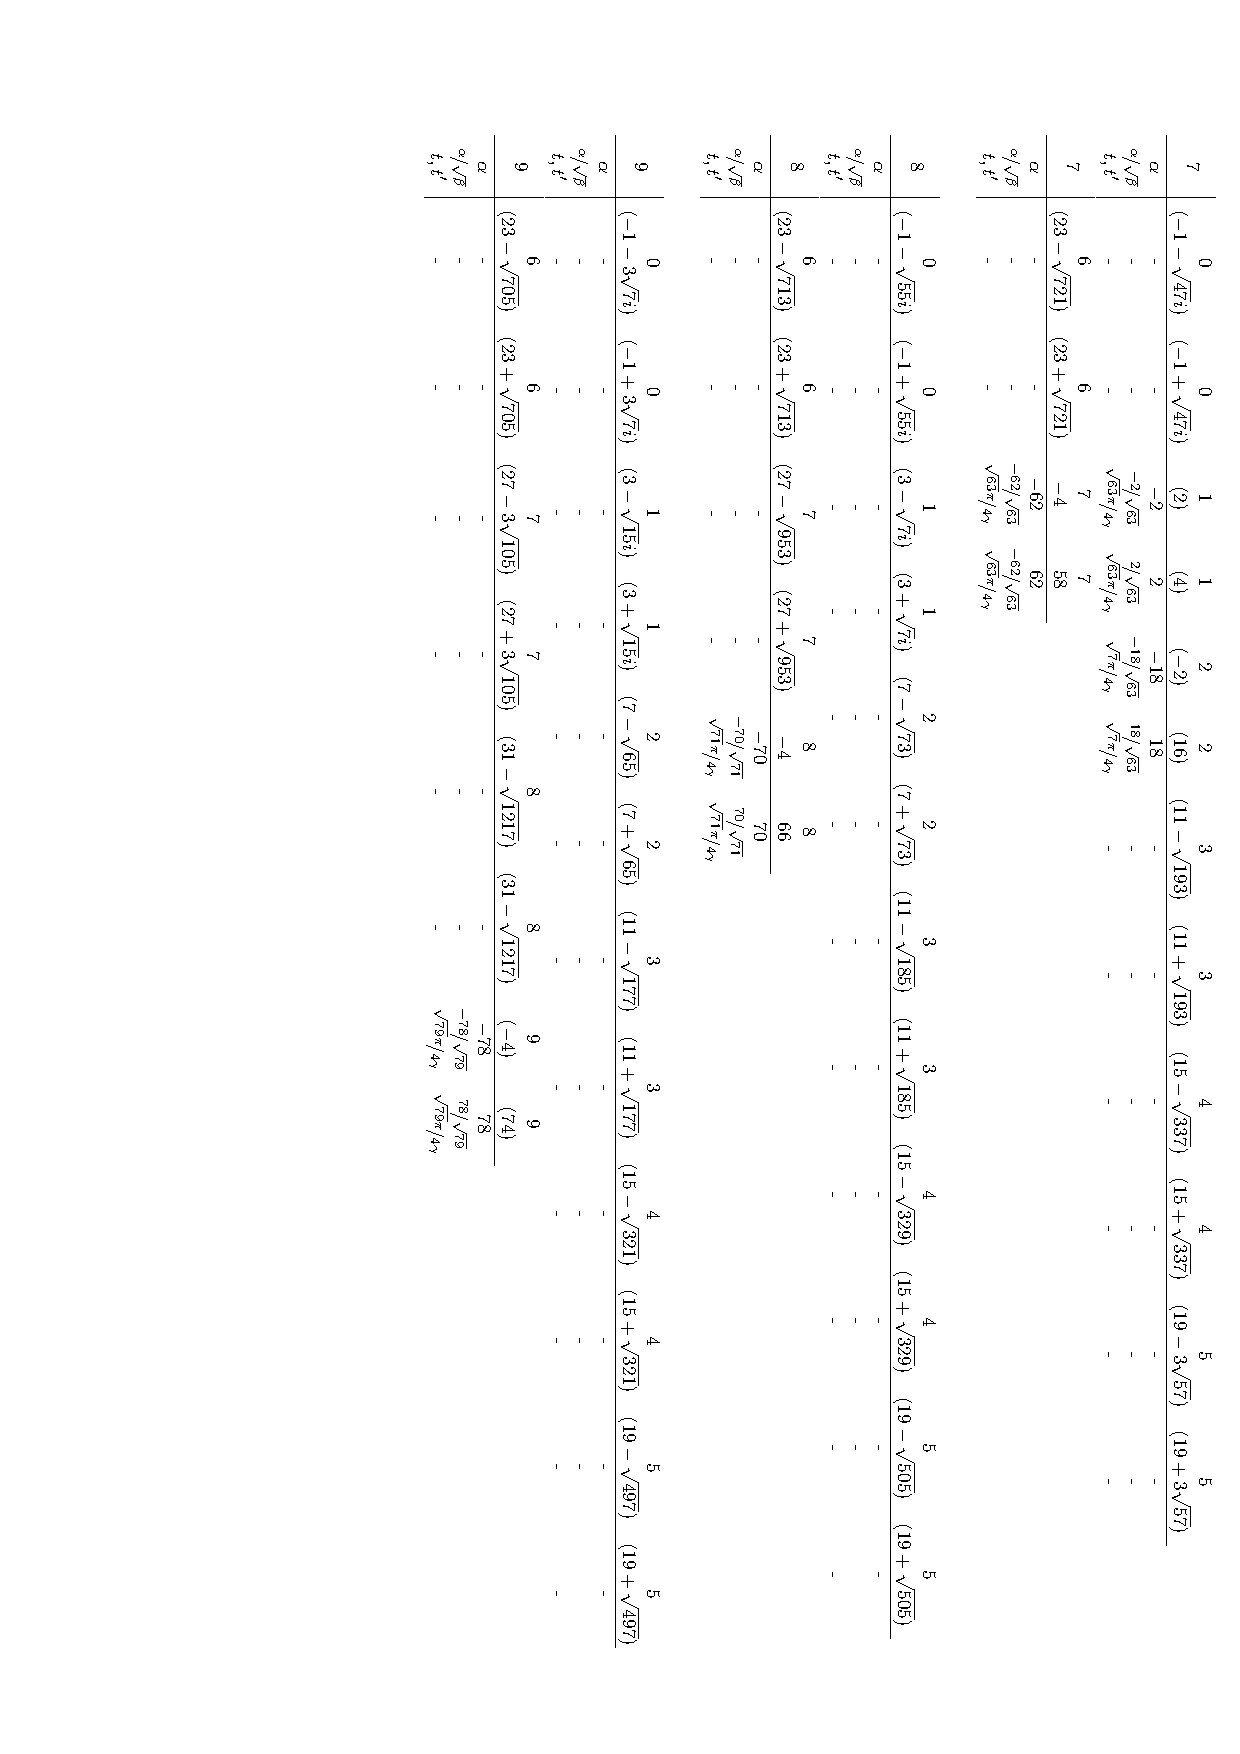
\includegraphics[width=\textwidth]{P4_PST_Node_1_to_Node_4 (2).pdf}
\end{center}
\FloatBarrier
\twocolumngrid
\bibliographystyle{unsrt}
\bibliography{references}
\end{document}